\section{Background and Overview}
\label{sec:overview}

This section starts with the introduction of the NUMA architecture and potential performance issues. Then it briefly discusses the basic idea of \NP{} to identify such issues. 

\subsection{NUMA Architecture}
\label{sec:numa}

Traditional computers use the Uniform Memory Access (UMA) model. In this model,  all CPU cores share a single memory controller such that any core can access the memory with the same latency (uniformly). However, the UMA architecture cannot accommodate the increasing number of cores because these cores may compete for the same memory controller. The memory controller becomes the performance bottleneck in many-core machines since a task cannot proceed without getting its necessary data from the memory. 

\begin{figure}[htbp]
%\vspace{-0.1in}
\centering
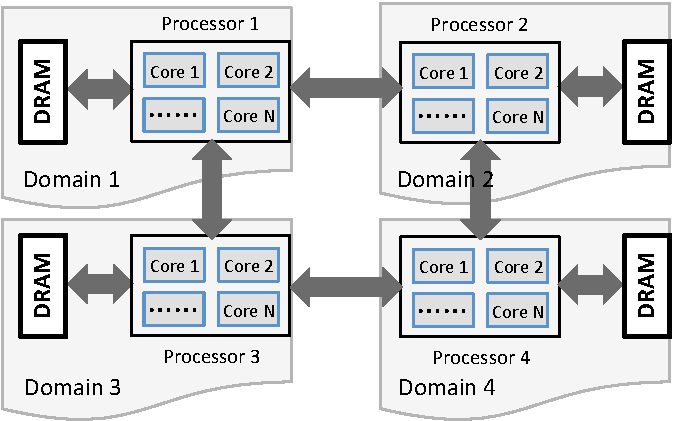
\includegraphics[width=0.9\columnwidth]{paper/figures/Numa.pdf}
\caption{A NUMA architecture with four nodes/domains\label{fig:numa}}
%\vspace{-0.1in}
\end{figure}

The Non-Uniform Memory Access (NUMA) architecture is proposed to solve this scalability issue, as further shown in Figure~\ref{fig:numa}. It has a decentralized nature. Instead of making all cores waiting for the same memory controller, the NUMA architecture is typically equipped with multiple memory controllers, where each controller serves a group of CPU cores (called a ``node'' or ``processor'' interchangeably). Incorporating multiple memory controllers largely reduces the contention for memory controllers and therefore improves the scalability correspondingly. However, the NUMA architecture also introduce multiple sources of performance degradations~\cite{Blagodurov:2011:CNC:2002181.2002182}, including \textit{Cache Contention}, \textit{Node Imbalance}, \textit{Interconnect Congestion}, and \textit{Remote Accesses}. 

\textbf{Cache Contention:} the NUMA architecture is prone to cache contention, including false and true sharing. False sharing occurs when multiple tasks may access distinct words in the same cache line~\cite{Hoard}, while different tasks may access the same words in true sharing. For both cases, multiple tasks may compete for the shared cache. Cache contention will cause more serious performance degradation, if data has to be loaded from a remote node. 
 
\textbf{Node Imbalance:} When some memory controllers have much more memory accesses than others, it may cause the node imbalance issue.
Therefore, some tasks may wait more time for memory access, thwarting the whole progress of a multithreaded application. 

\textbf{Interconnect Congestion:} Interconnect congestion occurs if some tasks are placed in remote nodes that may use the inter-node interconnection to access their memory. 

\textbf{Remote Accesses:} In a NUMA architecture, local nodes can be accessed with less latency than remote accesses. 
Therefore, it is important to reduce remote access to improve performance.



\subsection{Basic Idea}
\label{sec:idea}

 
Existing NUMA profilers mainly focus on detecting remote accesses, while omitting other performance issues. In contrast, \NP{} has different design goals as follows.  First, it aims to identify different sources of NUMA performance issues, not just limited to remote accesses. Second, \NP{} aims to design architecture- and scheduling-independent approaches that could report performance issues in any NUMA hardware. Third, it aims to provide sufficient information to guide bug fixes.  

For the first goal, \NP{} detects NUMA issues caused by cache contention, node imbalance, interconnect congestion, and remote accesses, where existing work only considers remote accesses.  \textit{Cache contention} can be either caused by false or true sharing, which may impose a larger performance impact and require a different fix strategy. Existing work never separates them from normal remote accesses. In contrast, \NP{} designs a separate mechanism to detect such issues by tracking possible cache invalidations caused by cache contention. 

It is infeasible to measure all \textit{node imbalance} and \textit{interconnect congestion} without knowing the actual memory and thread binding. Instead, \NP{} focuses on one specific type of issues, which is workload imbalance between different types of threads. 
Existing work omits one type of remote access caused by thread migration, where thread migration will make all local accesses remotely. 
\NP{} identifies whether an application has a higher chance of thread migrations, in addition to normal remote accesses. 
Overall, \NP{} detects more NUMA performance issues than existing NUMA profilers. However, the challenge is to design architecture- and scheduling-independent methods. 


The second goal of \NP{} is to design architecture- and scheduling approaches that do not bind to specific hardware. Detecting remote accesses is based on the key observation of Section~\ref{sec:intro}: \textit{if a thread accesses a physical page that was initially accessed by a different thread, then this access will be counted as remote access}. This method is not bound to specific hardware, since memory sharing patterns between threads are typically invariant across multiple executions. 
\NP{} tracks every memory access in order to identify the first thread working on each page. Due to this reason, \NP{} employs fine-grained instrumentation, since coarse-grained sampling may miss the access from the first thread. Based on memory accesses, \NP{} also tracks the number of cache invalidations caused by false or true sharing with the following rule: a write on a cache line with multiple copies will invalidate other copies. Since the number of cache invalidations is closely related to the number of concurrent threads, \NP{} divides the score with the number of threads to achieve a similar result with a different number of concurrent threads, as further described in Section~\ref{sec: cacheline}. Load imbalance will be evaluated by the total number of memory accesses of different types of threads. It is important to track all memory accesses including libraries for this purpose. To evaluate the possibility of thread migration, \NP{} proposes to track the number of lock contentions and the number of condition and barrier waits. Similar to false sharing, \NP{} eliminates the effect caused by concurrent threads by dividing with the number of threads. The details of these implementations can be seen in Section~\ref{sec:implementation} . 



For the third goal, \NP{} utilizes the data-centric analysis as in existing work~\cite{XuNuma}. That is, it could report the callsite of heap objects that may have NUMA performance issues. 
In addition, \NP{} aims to provide useful information that helps bug fixes, which could be easily achieved when all memory accesses are tracked. \NP{} provides word-based access information for cache contentions, helping programmers to differentiate false or true sharing. It provides threads information on page sharing (help determining whether to use block-wise interleave), and reports whether an object can be duplicated or not by tracking the temporal read/write pattern.
\NP{} also predicts a good thread assignment to achieve better performance for load imbalance issues. In summary, many of these features require fine-grained instrumentation in order to avoid false alarms. 


Due to the reasons mentioned above, \NP{} utilizes fine-grained memory accesses to improve the effectiveness and provide better information for bug fixes. \NP{} employs compiler-based instrumentation in order to collect memory accesses to address performance and flexibility concern. An alternative approach is to employ binary-based dynamic instrumentation~\cite{DynamoRlO, Valgrind, Pin}, which may introduce more performance overhead but without an additional compilation step. \NP{} inserts an explicit function call for each read/write access on global variables and heap objects, while accesses on stack variables are omitted since they typically do not introduce performance issues. To track thread migration, \NP{} also intercepts synchronizations. To support data-centric analysis, \NP{} further intercepts memory allocations to collect their callsites.  
\begin{figure}[!htbp]
\centering
\includegraphics[width=0.98\columnwidth]{figures/overview.pdf}
\caption{Overview of \NP{}\label{fig:overview}}
\vspace{-0.2in}
\end{figure}

Figure~\ref{fig:overview} summarizes \NP{}'s basic idea.  \NP{} includes two components, \NP{}-Static and \NP{}-Dynamic. \NP{}-Static is a static compile-time based tool that inserts a function call before every memory access on heap and global variables, which compiles a program into an instrumented executable file. Then this executable file will be linked to \NP{}-Dynamic so that \NP{} could collect memory accesses, synchronizations, and information of memory allocations. \NP{} then performs detection on NUMA-related performance issues, and reports to users in the end.  More specific implementations are discussed in Section~\ref{sec:implementation}. 
